\begin{frame}{Initialisierung}
    \begin{columns}[T] % T aligns the tops of the columns
        \begin{column}{0.75\textwidth}
            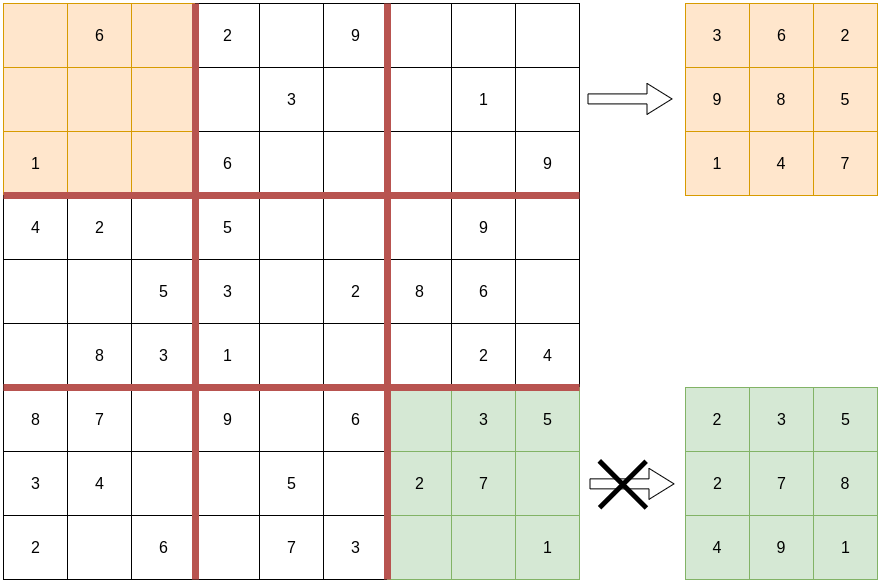
\includegraphics[width=\textwidth]{Pictures/Initialisierung.png}
        \end{column}
        \begin{column}{0.35\textwidth}
            \begin{itemize}
                \item zufällige Initialisierung leerer Felder
                \item einfache Methode: keine doppelten in Blöcken
                \item intelligente Initialisierung: möglichst keine doppelten in Zeilen
            \end{itemize}
        \end{column}
    \end{columns}
    \note[item]{generell Invariante: niemals Duplikate in Bloecken}
    \note[item]{gelb: moeglich trotz Kollision}
    \note[item]{gruen: nicht moeglich wegen K. im Block}
    \note[item]{einfach: komplett zufaellig}
    \note[item]{intelligent: moeglichst keine Kollisionen in Zeilen}
\end{frame}
